%%-------------------------------------------------------------------------------------- Início
\section{Controle de Versão}
\begin{frame}[allowframebreaks,fragile,t]{Configuração do Bitbucket e do Git}
  \begin{enumerate}
    \item Conecte-se o endereço \url{https://bitbucket.org} e crie uma conta neste servidor git,
      fornecendo usuário, e-mail e senha.
      \begin{figure}[h!]
	\centering
	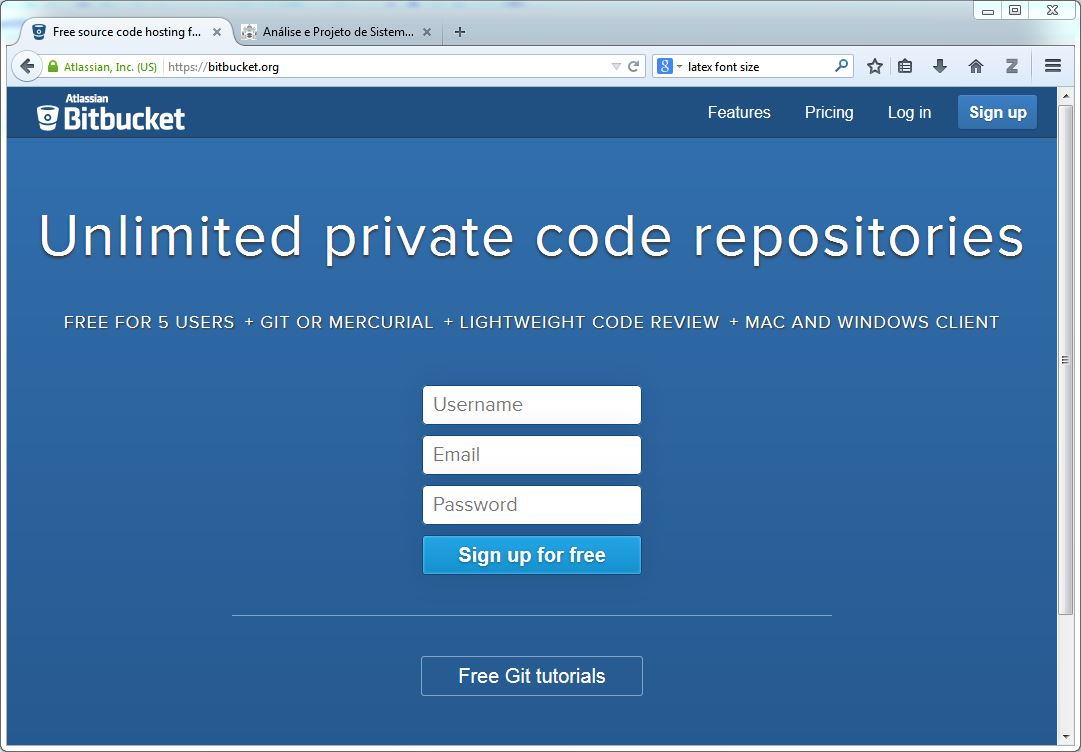
\includegraphics[width=0.45\textwidth]{devops/imagens/bitbucket-1.jpg}
      \end{figure}
      
     \framebreak
     \item Crie o repositório remoto, clicando na opção \verb!Repository->Create repository!.
      \begin{figure}[h!]
	\centering
	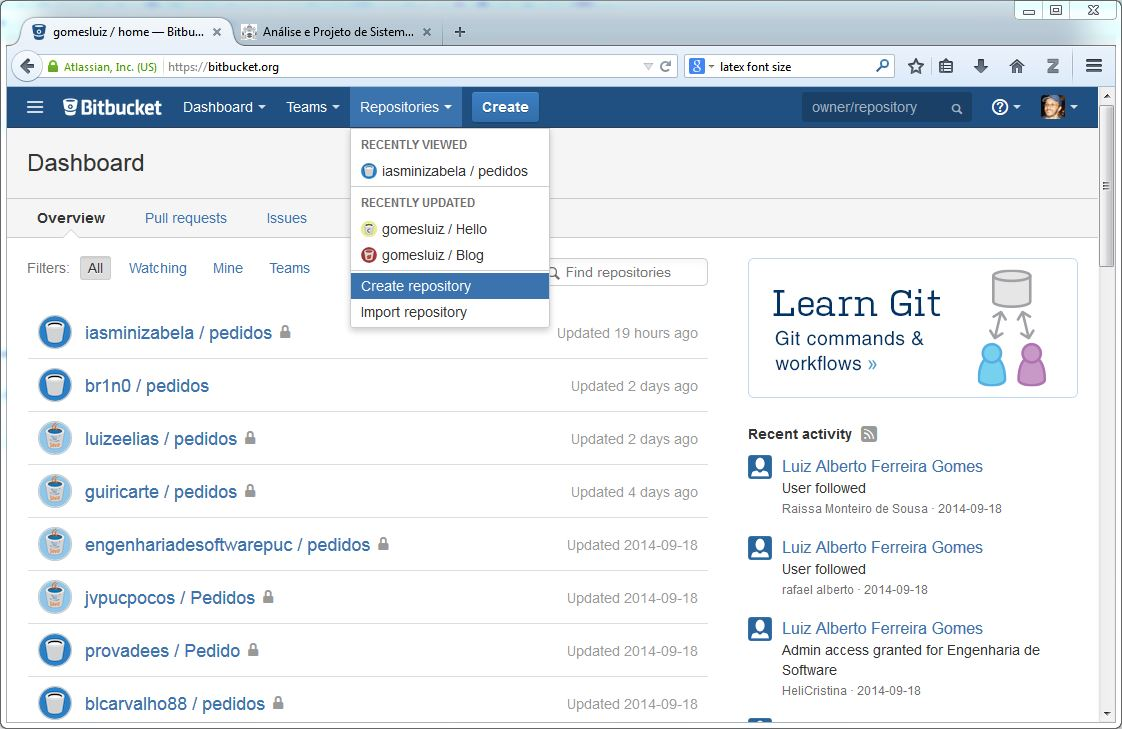
\includegraphics[width=0.45\textwidth]{devops/imagens/bitbucket-2.jpg}
      \end{figure}
      
     \framebreak
     \item Preencha o nome com \alert{do seu projeto}; assinale a opções \alert{Issue Tracking} e 
      \alert{Wiki}; e, por último, escolha como linguagem de projeto, por exemplo, \alert{Ruby}. Deixe
      as demais opções como estão e clique em \verb!Create repository!
      \begin{figure}[h!]
	\centering
	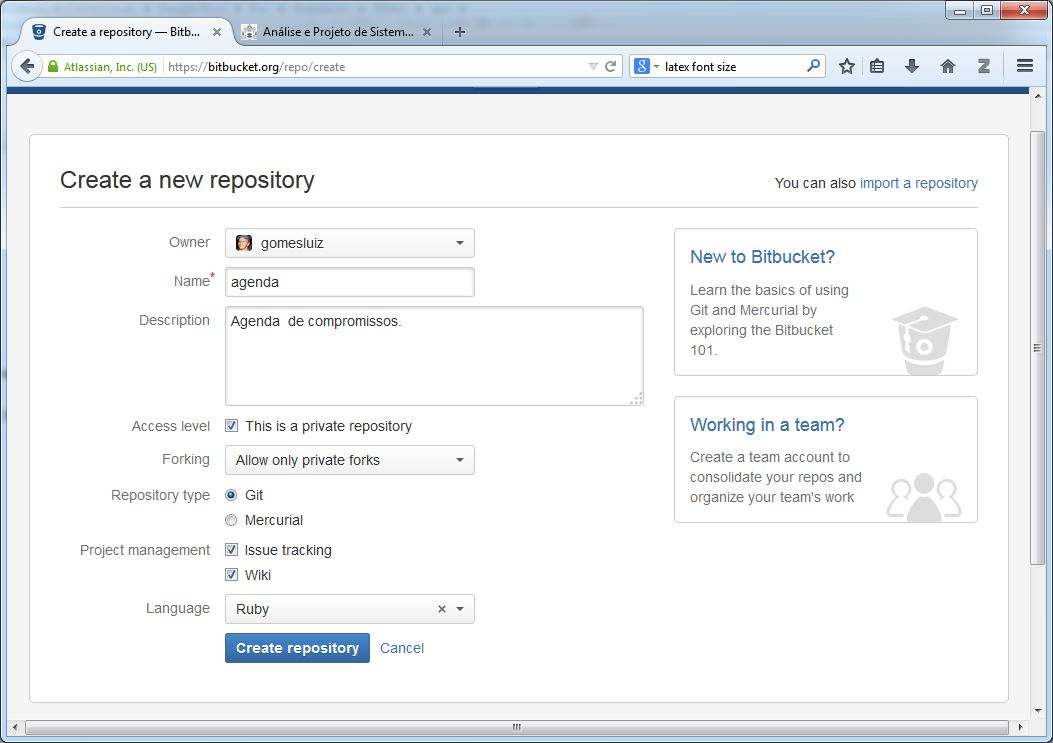
\includegraphics[width=0.45\textwidth]{devops/imagens/bitbucket-3.jpg}
      \end{figure}
      
      \framebreak
      \item Anote o endereço do seu repositório clicando no ícone \alert{. . .} e depois
	na opção \verb!Clone!. Precisaremos dele mais tarde.
      \begin{figure}[h!]
	\centering
	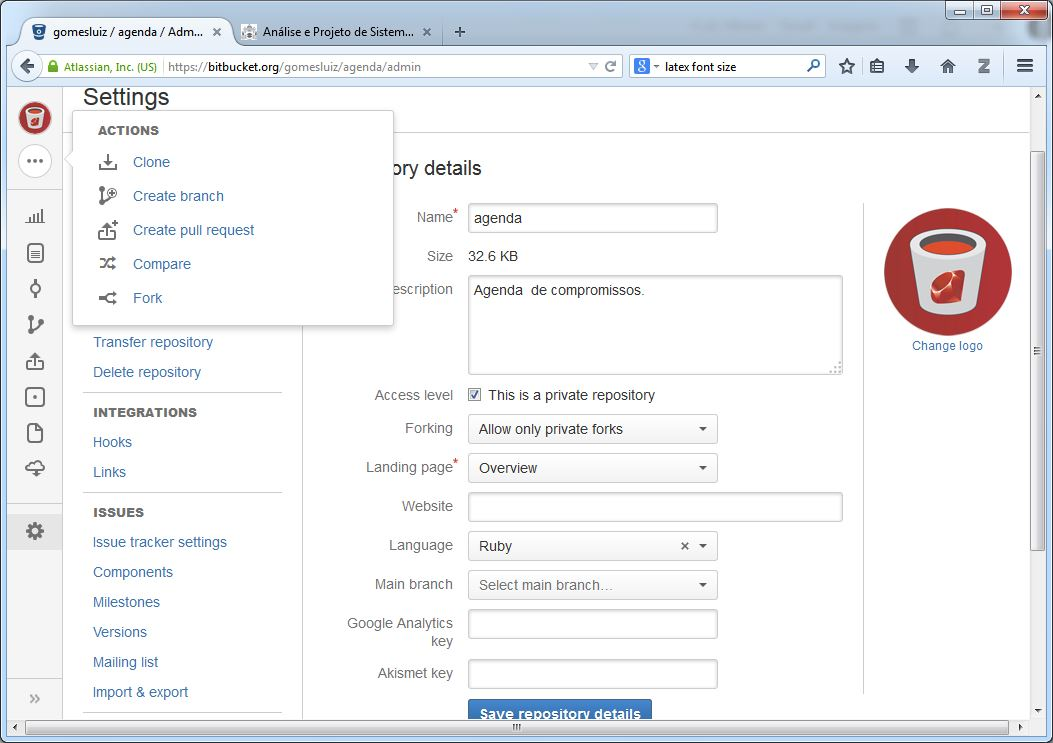
\includegraphics[width=0.45\textwidth]{devops/imagens/bitbucket-4.jpg}
      \end{figure}
      
      \framebreak
      \item O endereço do seu repositório começa em https, por exemplo, 
	\url{https://gomesluiz@bitbucket.org/gomesluiz/blog.git}
      \begin{figure}[h!]
	\centering
	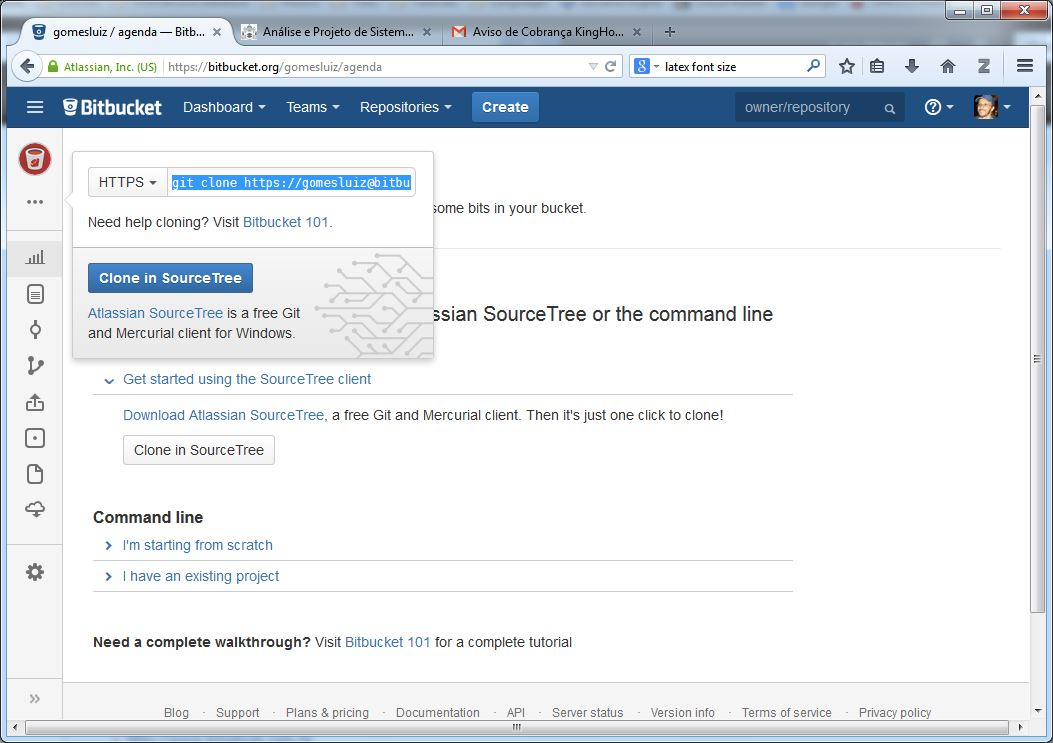
\includegraphics[width=0.45\textwidth]{devops/imagens/bitbucket-5.jpg}
      \end{figure}
      
      \framebreak
      \item Por último, configure o git localmente, digitando os comandos abaixo. Utilize
	o \alert{mesmo endereço} de e-mail utilizado para criar o repositório no Bitbucket.
      \begin{lstlisting}[style=BashInputStyle]      
	  $ git config --global color.ui true
	  $ git config --global user.name "Seu Nome"
	  $ git config --global user.email "seu@email.com"
      \end{lstlisting}
      
			\item Inicialize o repositório git local.
			\begin{lstlisting}[style=BashInputStyle]
				$ cd ~/Workspace/<nome do projeto>
				$ git init
			\end{lstlisting}
			
			\item Inclua todos os arquivos da aplicação no repositório local e efetive 
			a gravação deles.
			\begin{lstlisting}[style=BashInputStyle]
				$ git add .
				$ git commit -m "Initial commit."
			\end{lstlisting}
			
			\item Vincule o repositório local ao repositório remoto no Bitbucket.org.
			\begin{lstlisting}[style=BashInputStyle]
				$ git remote add origin EnderecoDoSeuRepositorio
			\end{lstlisting}
			
			\item Envie os arquivos do repositório local para repositório remoto no Bitbucket.org utilizando
			o comando a seguir e, após isso, visualize-os no \verb!Dashboard! do \url{http://bitbucket.org}.
			\begin{lstlisting}[style=BashInputStyle]
				$ git push -u origin master
			\end{lstlisting}
			
  \end{enumerate}
\end{frame}
